 
 \vspace*{0.5cm}
 

 \begin{center}
 	
 	\shadowoffset{2pt}
 	\shadowrgb{0.7,0.7,0.7}
 	
	 \begin{blueshaded}
	 	\begin{center} 
	 	\vspace{0.5cm}
	 			
		{\fontfamily{phv}\fontsize{38}{57}\selectfont 
			\textbf{\shadowtext{Matemàtiques 3r ESO}} 
		}
		 
		\vspace{1cm}
		\shadowoffset{1pt}
		{\huge \textbf{\shadowtext{Sèrie Pràctica}}}
	
		\vspace{1cm}
	
	{\Large \normalfont\textit{2a Edició}	}	
		\vspace{0.5cm}
\end{center}

\end{blueshaded}
 

 \vspace{1cm}
 
 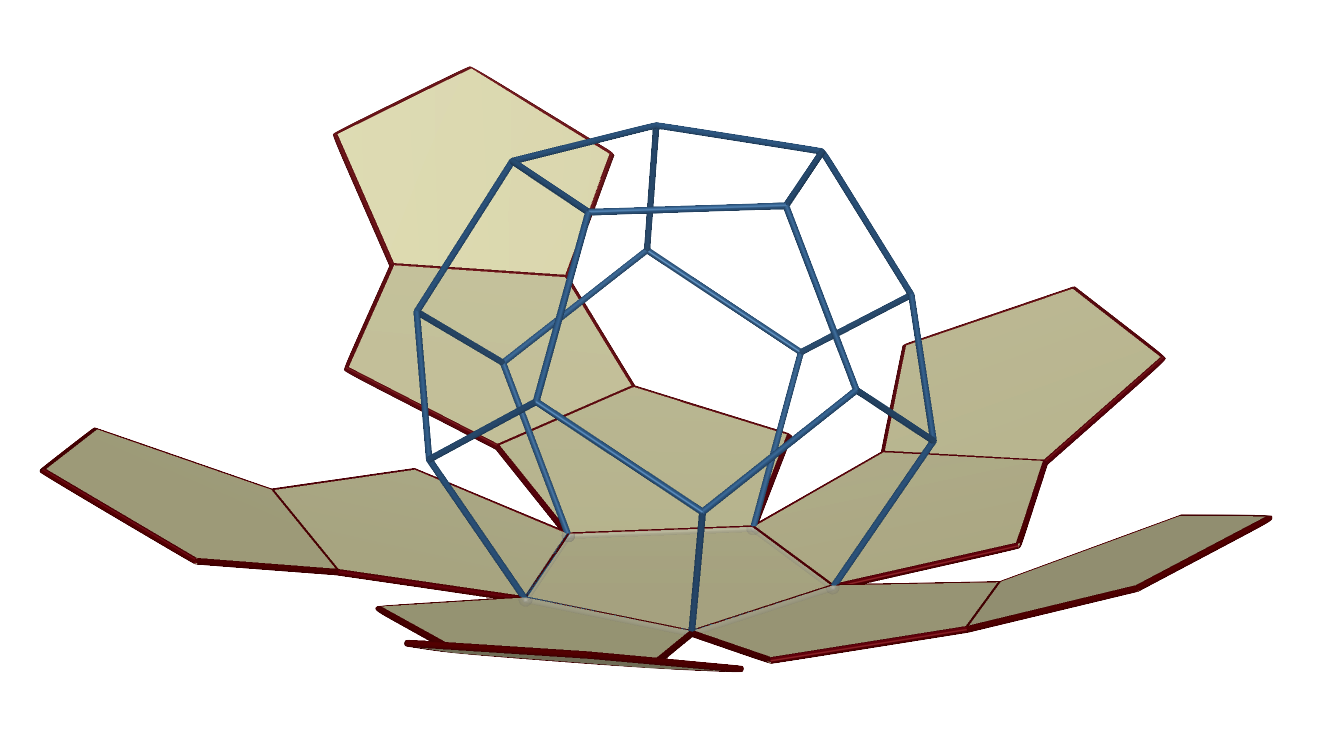
\includegraphics[width=0.9\textwidth]{img-00/portada}

\vspace{1.5cm}

 
\begin{minipage}{0.4\textwidth}
\begin{center}
	\includegraphics*[width=1.2in]{img-00/ies-binissalem-logo}
 
	\small
	
	\noindent \href{www.iesbinissalem.net}{\textbf{www.iesbinissalem.net}}  
 
\end{center}
\end{minipage}
\begin{minipage}{0.4\textwidth}
\begin{flushright}
\textbf{Josep Mulet}

\textit{Departament de Matemàtiques} 

 IES Binissalem
\end{flushright}
\end{minipage} 


\end{center}

\newpage

\vspace*{12.5cm}
 \begin{center}
 	\begin{minipage}{0.5\textwidth}
 		Aquesta és una obra derivada de ``\textit{Matematicas 3º de ESO. Ejercicios y problemas}'' de Marea Verde de matemàtiques. Per tant, està subjecta a les mateixes condicions de llicència CREATIVE COMMONS que l'obra original.
 		
 		 \noindent \textbf{Edició \LaTeX: \quad \textregistered \,  Josep Mulet Pol}
 		
 		 \noindent \textbf{Versió}: \quad 2017-07-23
 		 
 		 \noindent \textbf{Portada}: \quad \textit{Desenvolupament d'un dodecaedre}.
 		 
 		
 		\begin{center}
 		\includegraphics*[width=8cm]{img-00/licencia}
 		\end{center}
 	\end{minipage}
 \end{center}
 
%\clearemptydoublepage
%%\setcounter{page}{1}
%%\fancyfoot[C]{\roman{\thepage}}%

\renewcommand{\thepage}{\Roman{page}}% Roman numerals for page counter
\pagestyle{myheadings}
\thispagestyle{empty}
\renewcommand{\headrulewidth}{0pt}
\renewcommand{\footrulewidth}{0pt}

\pagebreak


\dominitoc

\tableofcontents

\newpage

\vspace*{\fill}
\begin{center}
	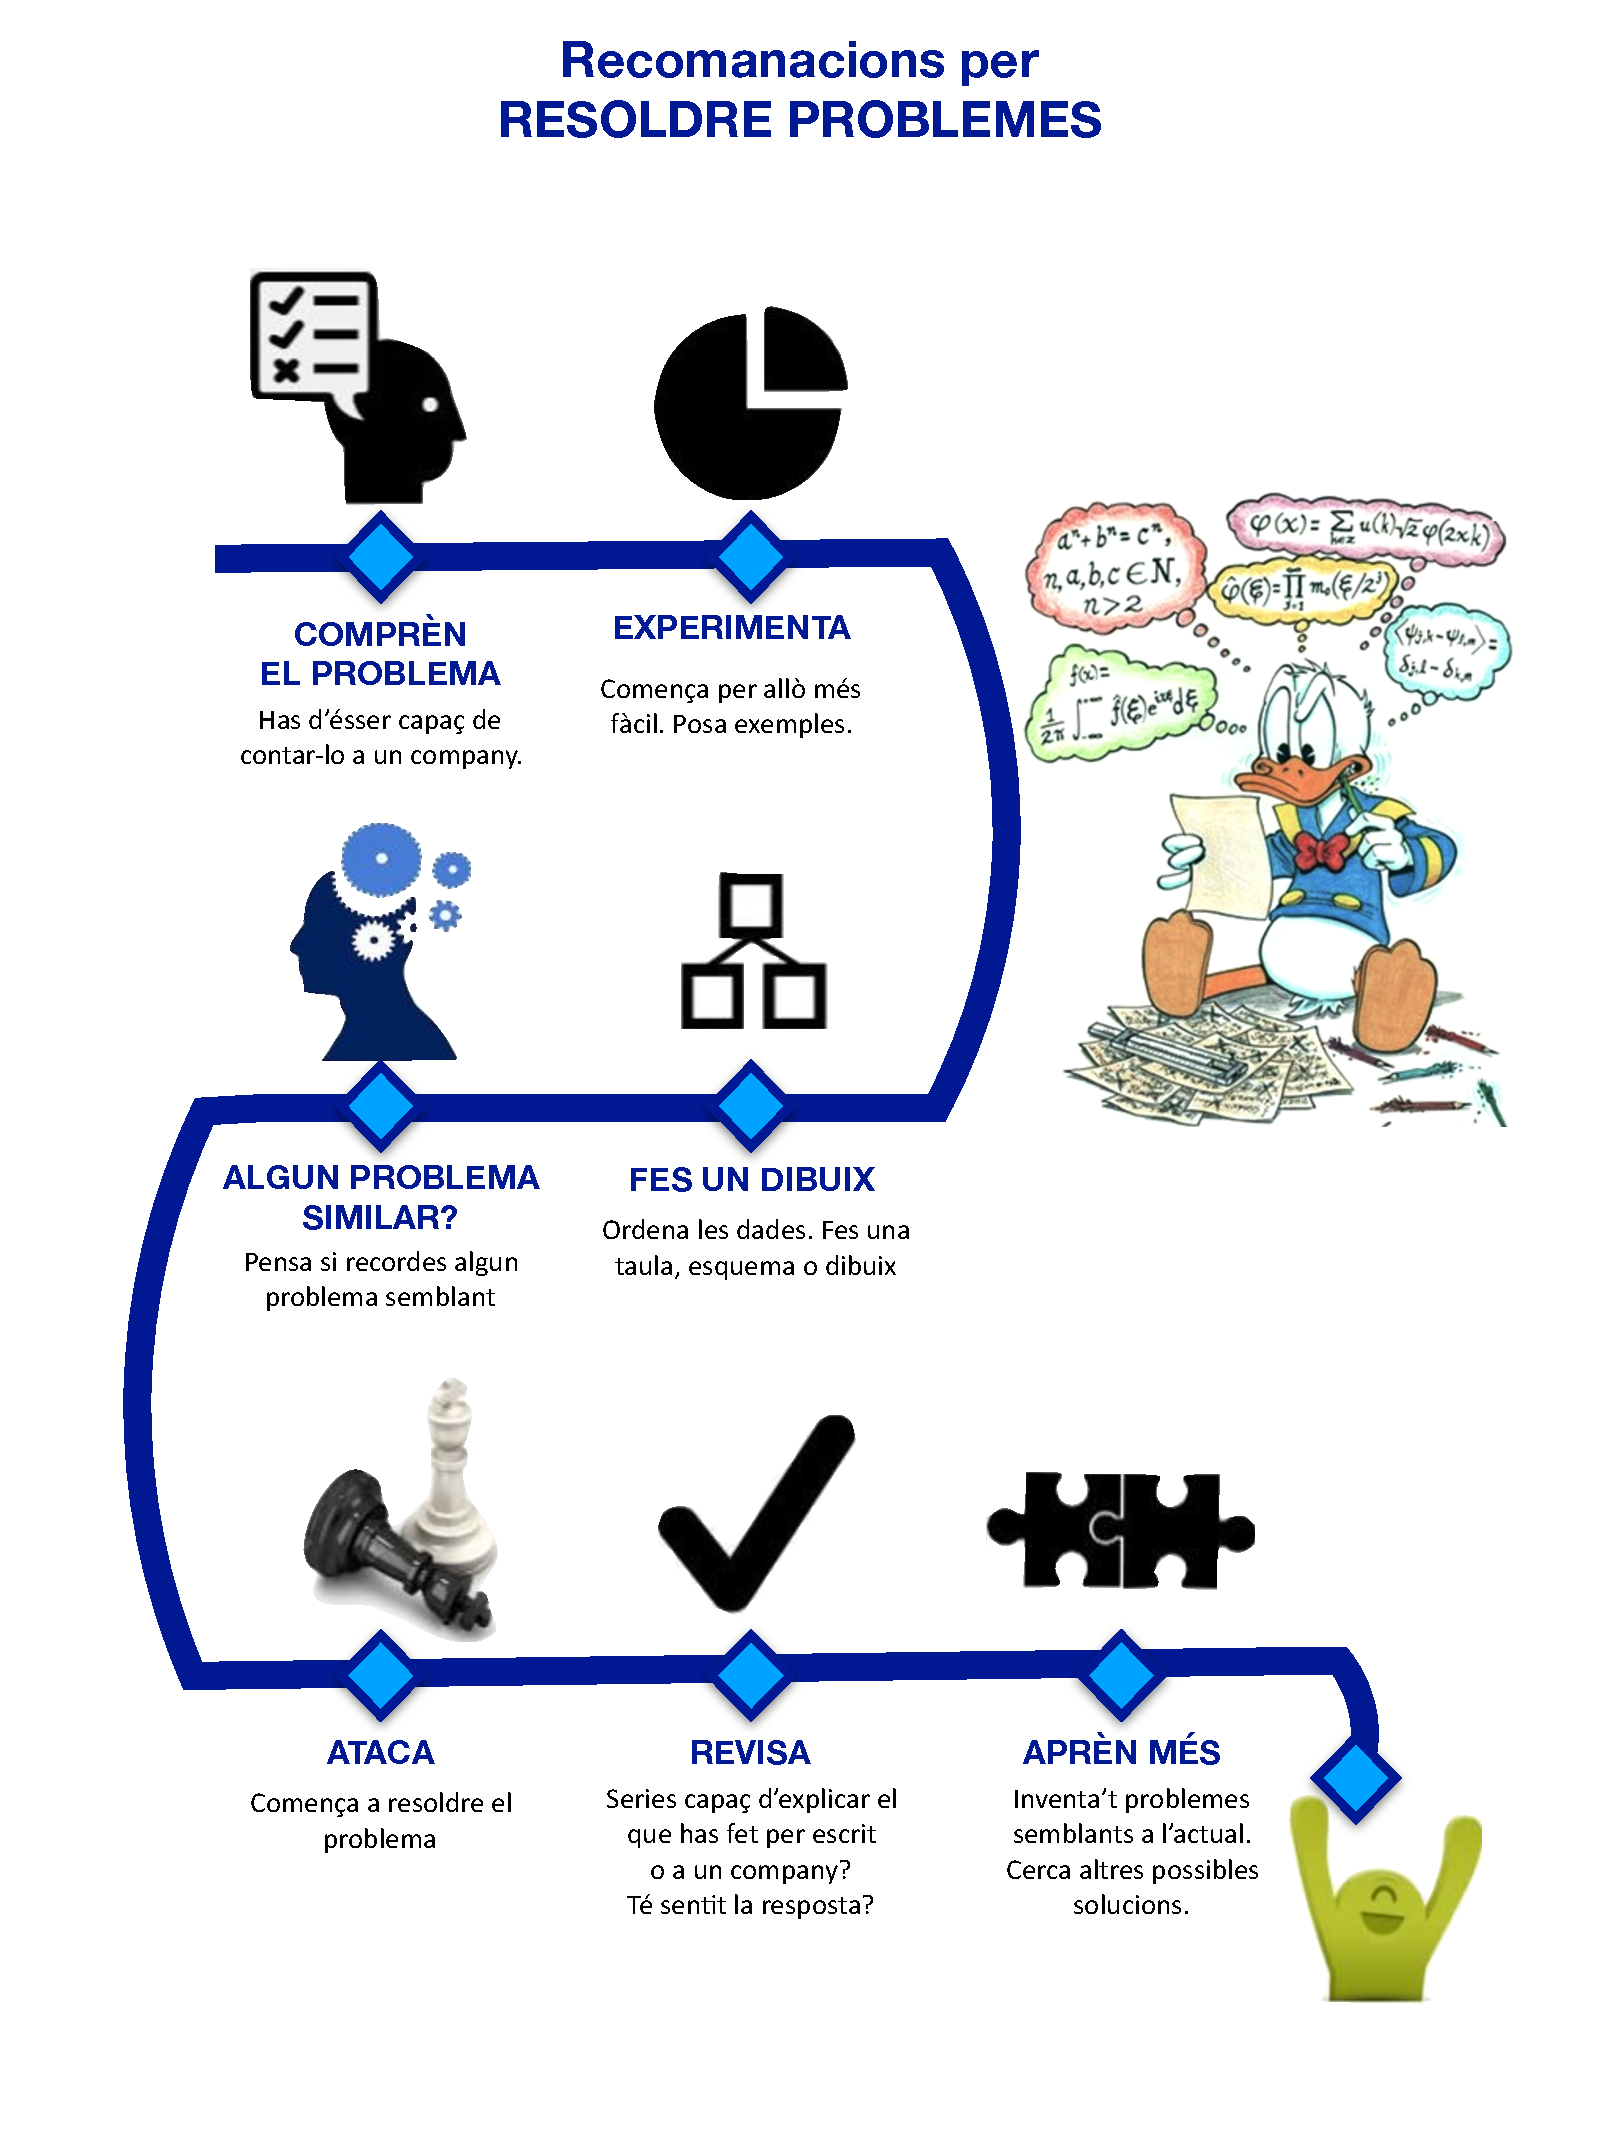
\includegraphics[width=\textwidth]{img-00/resolucio-problemes}
\end{center}
\vspace*{\fill}



\cleartorightpage


\vspace*{2cm} 
\heading{Símbols}

\begin{center}
	\renewcommand{\arraystretch}{1.5}
\begin{longtable}[h]{>{\raggedleft\arraybackslash}p{0.19\textwidth}|p{0.78\textwidth}}
	{\bfseries Símbol} & {\bfseries Significat} \\ \hline
	
	\simbolclau & Problema clau amb solució al final del llibre.  \\ \hline
	
	\simbolcompass & A més de la solució, proporciona orientacions per arribar a ella.  \\ \hline
	
	\simbolsearch & Problema que requereix d'investigació o recerca d'informació.  \\ \hline

	\ggb & Activitat adequada per realitzar amb el programa Geogebra.  \\ \hline
		
	\begin{center}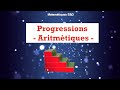
\includegraphics[width=1cm]{img-00/video-132}\par {\footnotesize Vídeo 132:}\end{center} & Explicació en vídeo dels continguts de l'apartat. El número de vídeo correspon a la numeració emprada en https://piworld.es 
	
	\\ \hline
	\hot[2] & Problema amb un cert grau de dificultat. \\ [0.25cm] \hline
	\spen & Activitat que es pot contestar en el llibre mateix. \\ [0.25cm] \hline 
	\mental & Activitat que es pot resoldre mentalment o en veu alta.
\end{longtable}
\end{center}
\vspace{1cm} 
 
\heading{Recursos}

\begin{center}
	\renewcommand{\arraystretch}{1.5}
\begin{longtable}[h]{>{\raggedleft\arraybackslash}p{0.2\textwidth}|p{0.8\textwidth}}
	\hline
	\textbf{piWorld}
	
	
\includegraphics[height=1.5cm]{img-00/piworld}
	 & Plataforma d'aprenentatge. Conté explicacions en vídeo i activitats interactives. Requereix usuari i contrasenya. \newline
	\href{https://piworld.es}{\href{https://piworld.es}{https://piworld.es}}
	\\ \hline
 	\textbf{Geogebra} 
 	
 	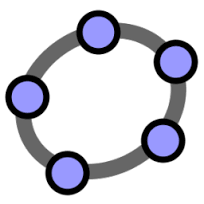
\includegraphics[height=1.5cm]{img-00/geogebra}
 	& Programa lliure de geometria dinàmica en dues i tres dimensions.
 	Ideal pels temes de funcions i geometria.\newline
 	\href{https://www.geogebra.org/download}{\href{https://www.geogebra.org/graphing}{https://www.geogebra.org/graphing}}
 	  \\ \hline
 	  	\textbf{Calculadora WIRIS}
 	 
 	  	
 	  	
\includegraphics[height=2cm]{img-00/wiris}
 	  	& Calculadora per al càlcul simbòlic. Nova versió Web \par \href{https://calcme.com/a}{https://calcme.com/a}
 	  	
 	  	La versió antiga la trobareu a \par \href{http://www.wiris.net/educa.madrid.org/wiris/es/cas.html}{http://www.wiris.net/educa.madrid.org/wiris/es/cas.html}
 	  	
 	  	 Atenció: requereix el plugin de Java i no funciona en dispositius mòbils.
 	  \\ \hline
 
 \end{longtable}
\end{center}
 